\documentclass[a4paper,12pt]{article}
\usepackage[T1]{fontenc}
\usepackage[utf8]{inputenc}
\usepackage{lmodern}
\usepackage{amsmath}
\usepackage{amsfonts}
\usepackage{amssymb}
\usepackage{amsthm}
\usepackage{graphicx}
\usepackage{color}
\usepackage{xcolor}
\usepackage{url}
\usepackage{theorem}
\usepackage{textcomp}
\usepackage{listings}
\usepackage{hyperref}
\usepackage{parskip}

\title{Motivace vzniku pocitace}
\author{Vojtech Vasek}

\begin{document}

\begin{center}
    \huge{\underline{\textbf{Motivace vzniku pocitace}}}
\end{center}

\begin{itemize}\item{algoritmus - presny navod ci postup, kterym lze vyresit dany typ úlohy.}\end{itemize}

\section{Motivace}
    \begin{itemize}
        \item{zprvu pomoc se slozitymi vypocty, pozdeji kancelarske prace jako jsou textove dokumenty a tabulky}
        \item{zautomatizovani neustale opakujicich se praci - clovek pri neustale stejne cinnosti chybuje}
    \end{itemize}

\section{Prvni mechanicke pocitace}
    \subsection{Abakus}
        \begin{itemize}
            \item{jednoduche pocitadlo s posuvnymi kulickami}
            \item{Vznikl pred asi 5 000 lety v Babylonii jako deska s kaminky. Slovo abakus se sklada ze slova *abaq* nebo-li *prach*. Ve starovekem recku a rime pouzivali hlinenou desku do ktere vkladaly kaminky (*calculli*)}
            \begin{figure}[htp]
                \centering
                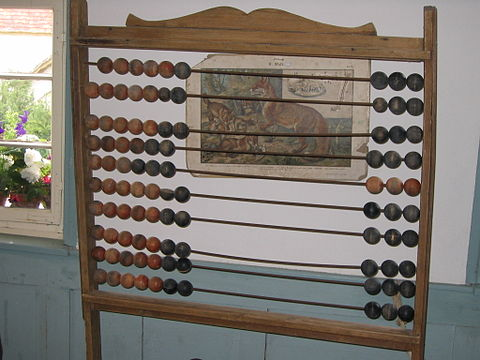
\includegraphics[width=8cm]{TVP_11_9_23@2.jpg}
            \end{figure}
        \end{itemize}
    \subsection{Logaritmicke tabulky a pravitko}
        \begin{itemize}
            \item{V roce 1614 byla objevena nova metoda nasobeni a deleni za pomoci scitani a odcitani. Po objeveni se v Anglii zacali stavet prvni tabulky.} 
            \item{Po tabulkach prisli logaritmicka pravitka, ktera se pouzivala dalsich 200 let (do 70. let 20. st.) ve skolach a v technickych oborech. Pri praci s velkymi cisly byla presnost mensi z důvodu zaokrouhlovani. Skladalo se ze dvou pohyblivych casti. Soucin bylo mozno vypocitat souctem logaritmů cisel vyznacenych na pravitku.}
            \begin{figure}[htp]
                \centering
                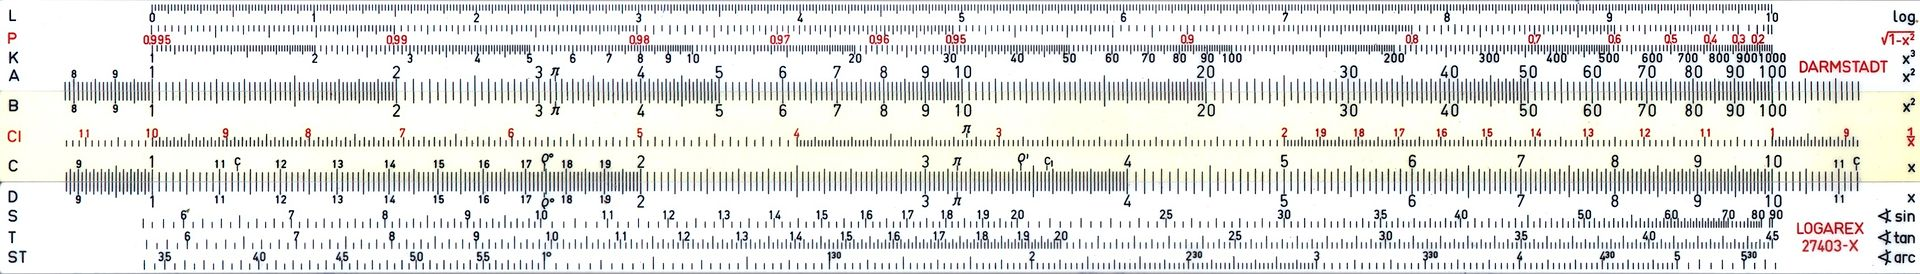
\includegraphics[width=8cm]{TVP_11_9_23@3.jpg}
            \end{figure}
        \end{itemize}
    \subsection{Mechanicke kalkulatory}
        \begin{itemize}
            \item{Prvni mechanicky kalkulator vynalezen mezi 150 az 100 lety pr. n. l. byl Mechanismus z Antikythery slouzil pravdepodobne k vypoctu polohy Slunce, Mesice a planet. Skladal se z triceti a vice ozubenych kolecek.}
            \item{Roku 1623 Schickard sestavil mechanicky kalkulator vyrobeny z ozubenych kolecek z hodin. Umel scitat a odcitat sesticiferna cisla.}
            \item{Dalsi pocitaci stroj byl vyroben Pascalem roku 1642 ktery umel take jen scitat a odcitat.  Roku  cca 1820 vytvoril Thomas prvni mech. kalkulator ktery umel scitat, odcitat, nasobit a delit. Byl take i seriove vyraben.}
            \item{Vetsina kalkulatorů byla stavena na desitkove soustave, ktera se obtizne implementovala.}
            \item{Nasledovaly derne stitky a tkalcovske stavy.}
        \end{itemize}
        
\section{Prvni programovatelne stroje}
    \begin{itemize}
        \item{roku 1833 Charles Babbage predbehl svou dobu vyvojem "Analytickeho stroje" ktery nemohl ve sve dobe vyrobit. Analyticky stroj se stal prvnim univerzalnim Turingovsky úplnym pocitacem *(lze napodobit jine pocitace bez nutnosti fyzicky upravit pocitac)* . Jeho pocitac mel pracovat s pevnou desetinnou carkou a padesati-mistnymi cisly. Mel mit "sklad" *(pamet)* a "mlynici" *(procesor)*. Programy byly psane do dernych stitků.}
        \begin{figure}[htp]
            \centering
            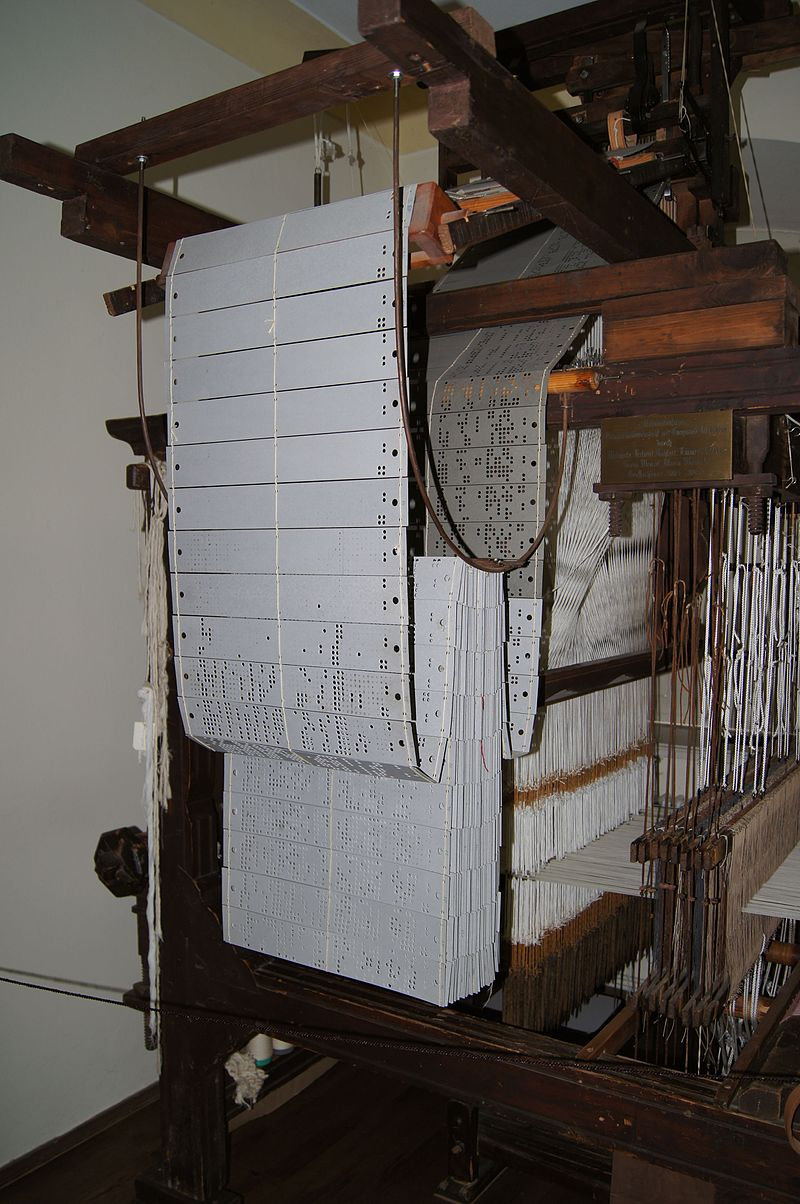
\includegraphics[width=4cm]{TVP_11_9_23@4.jpg}
        \end{figure}
    \end{itemize}
    
\section{Nulta generace}
    \begin{itemize}
        \item{prvni pocitace teto generace ve vetsine pripadů jiz pouzivala rele a pracovaly na kmitoctu +- 100 Hz. Diky druhe svetove valce se tato oblast techniky vyrazne posunula vpred.}
    \end{itemize}
    \subsection{Z1}
        \begin{itemize}
            \item{prace na konstrukci zacala jiz roku 1934 a dokoncena byla roku 1936. stroj pracoval v dvojkove soustave a neumel podminene skoky. programy se psaly na derne pasky (nosicem byl kinofilm). cely elektromechanicky stroj byl dokoncen az roku 1938. byl velmi poruchovy tudiz prakticky nepouzitelny. povazovan za prvni pocitac.}
        \end{itemize}
    \subsection{Z2, Z3}
        \begin{itemize}
            \item{po dokonceni Z1 se nemecky inzenyr Zuse vrhl na Z2 ktery mel 200 rele a mechanickou pameť ze Z1.}
            \item{Nasledovala spoluprace Zuseho a Schreyre pro vytvoreni jeste vykonnejsiho pocitace Z3. Z3 byl znicen pri naletech v roce 1944}
        \end{itemize}
    \subsection{ABC}
        \begin{itemize}
            \item{v rijnu 1939 sestavil americky profesor Atanasoff elektronicky pocitac ABC, ktery slouzil k reseni linearnich rovnic ve fyzice.}
        \end{itemize}
    \subsection{Colossus}
        \begin{itemize}
            \item{Colossus MK1 byl zkonstruovan roku 1943 Thomasem H. Flowers jako prototyp desifrovaciho pocitace pouzit pro desifrovani textu strojem Enigma. Pouzival vakuove elektronky.}
            \item{Colossus MK2 byl zkonstruovan o rok pozdeji pro desifraci zprav zasifrovane pristrojem Lorenz cipher.}
        \end{itemize}
    \subsection{SAPO}
        \begin{itemize}
            \item{Prvni pocitac vyrobeny v ceskoslovensku. Nazev SAPO je zkratkou pro SAmocinny POcitac. Byl uveden do provozu roku 1957 a obsahoval 7 000 rele a 400 elektronek. Byl zvlastni ve dvou vecech: soucasti kazde instrukce bylo 5 adres (2 operandy, vysledek, adresy skoku v pripade kladneho a zaporneho vysledku) a mel 3 procesory, ktere pracovaly paralelne.}
            \item{O spravnosti vysledku se hlasovalo. Vysledek z kazdeho procesoru se porovnaval, pokud se alespoň vysledek jednoho procesoru shodoval s vysledkem druheho procesoru vysledek byl prohlasen za spravny; pokud se vsechny tri vysledky neshodovaly, proces se opakoval.}
            \item{Tri roky po svem spusteni SAPO shorel. Z jiskricich releovych kontaktů se vzňala louzicka oleje, kterym se rele promazavala.}
        \end{itemize}

\section{Prvni generace}
    \begin{itemize}
        \item{prvni generace jiz pouzivala elektronky (rele jen v mensi mire). Pocitace byly vysoce poruchove, neefektivni a prilis nakladne. Nemeli zadny operacni system ani progr. jazyky, programy se psaly na propojovaci desky, pozdeji na derne stitky a pasky. Byly vybaveny tiskarnou pro vytisk vysledku na derny stitek. Za úspech se povazovalo ukoncit vypocet bez poruchy pocitace.}
    \end{itemize}
    \subsection{ENIAC a MANIAC}
        \begin{itemize}
            \item{Roku 1944 na univerzite v Pensylvanii uveden do provozu elektronicky pocitac EINAC. Na rozdil od Z3 umozňoval vytvoreni smycky i podminene skoky a byl Turingovsky úplny. Provadel az 5000 souctů za sekundu, ale byl energeticky velmi narocny, poruchovy a jeho provoz byl drahy.}
            \item{MANIAC byl inspirovan od ENIACu, sestaven roku 1945 a zprovoznen roku 1952. Byl vyuzit k matematickym vypoctům popisujici fyzikalni deje a k vyvoji jadernych bomb.}
        \end{itemize}

\section{Druha generace}
    \begin{itemize}
        \item{druha generace pouziva polovodicove soucastky - tranzistory. To zapricinilo zrychleni, zmenseni a spolehlivost pocitace ale i snizeni energetickych naroků.}
        \begin{figure}[htp]
            \centering
            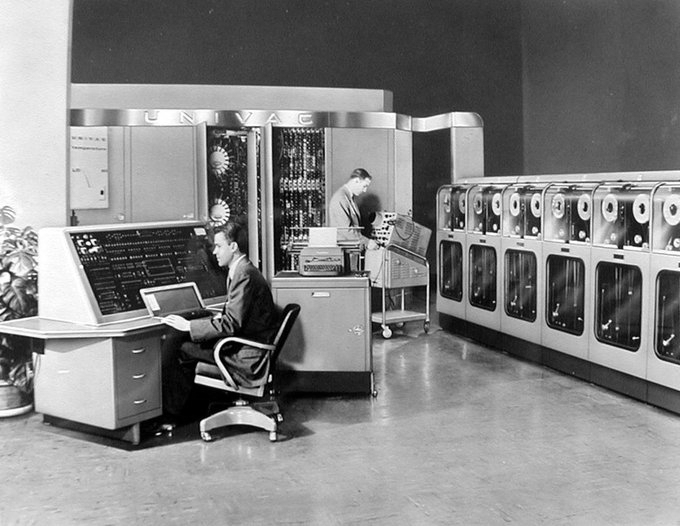
\includegraphics[width=8cm]{TVP_11_9_23@5.jpg}
        \end{figure}
    \end{itemize}
    \subsection{UNIVAC}
        \begin{itemize}
            \item{v roce 1951 prvnim seriove vyrabenym komercnim pocitacem. Paty vyrobeny kus úspesne predpovedel vysledky voleb.}
        \end{itemize}
    \subsection{EPOS (1 a 2)}
        \begin{itemize}
            \item{Roku 1960 byl spusten EPOS 1. Pracoval v desitkove aritmetice, v kódu, ktery umozňoval automatickou opravu jedne chyby. V 60. a 70. letech se vyrabel i v mobilni verzi a byl vybaven operacnim systemem, assemblerem a prekladacem.}
            \item{EPOS 2 byl spusten dva roky po EPOS 1. Byl osazen tranzistory a konstruovan do stavebnicove formy - pro kazdy typ vyuziti se dal sestavit "optimalni system".}
        \end{itemize}

\section{Treti generace}
    \begin{itemize}
        \item{Jiz pouzivala integrovane obvody. Zacalo se objevovat multiprogramovani - zatimvo jeden program ceka na dokonceni I/O operace, je procesorem zpracovavana druha úloha. Objevuje se take novy termin proces, prvni podpra multitaskingu. Krom velkych pocitaců pres celou mistnost (mainframe) se objevuji prvni mini- a mikropocitace.}
    \end{itemize}
    \subsection{IBM System 360}
        \begin{itemize}
            \item{Objevil se v různych vykonnostnich modelech, od modelu 360/20 az po 360/90, a vsechny mohly pouzivat shodny software. mohly pracovat jak s pevnou, tak take promennou delkou operandů (dat). Vyrabeli se v tisicovych serii, a byly obrovskym pokrokem v komercnim vyuziti.}
        \end{itemize}
    \subsection{Cray}
        \begin{itemize}
            \item{tehdy nejvykonnejsi pocitac na svete Cray-1 (prvni superpocitac). S nastupem paralelnich vypoctů Cray-1 ustoupil a firma v roce 1995 zkrachovala.}
        \end{itemize}

\section{ctvrta (dnesni) generace}
    \begin{itemize}
        \item{Charakterizuje ji mikroprocesory a osobni pocitace. Zmensil se procesor (drive slozeny z nekolika obvodů), zvysila se rychlost, spolehlivost a kapacita pameti, snizila se velikost a naklady. Zacinaji ustupovat mainframey a nahrazuji je osobni stolni pocitace (v roce 1981 uveden IBM PC) a laptopy. Ostatni vyrobci zacinaji vyrabet pocitace shodne konstrukce jako "IBM PC kompatibilni". Prichazi era GUI, DOSu (prevazne MS-DOS), pozdeji MS Windows (zprvu postavene na DOSu, pozdeji na NT) a jinych operacnich systemu jako je *System 1-9*, pozdeji nahrazen*macOS*, Unix/BSD, GNU/Linux, BeOS/Haiku, OS/2.}
        \begin{figure}[htp]
            \centering
            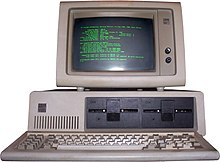
\includegraphics[width=8cm]{TVP_11_9_23@6.jpg}
        \end{figure}
    \end{itemize}
    
\section{Budoucnost}
    \begin{itemize}
        \item{zatim se nevi jakym smerem se vyvoj bude ubirat.}
        \item{prvni komercni kvantovy pocitac IBM Q System One byl predstaven v lednu 2019.}
    \end{itemize}

\end{document}